\documentclass[mathserif]{beamer}
%\documentclass{beamer}
\usetheme{Luebeck}
\usecolortheme{spruce}
\usecolortheme{rose}
\usepackage{amsmath,verbatim}
\usepackage{listings}
\usepackage[english]{babel}
%\usepackage{media9} % package for genuine embedding of movies
%\usepackage{multimedia} % beamer package for calling external files and players
\setbeamercovered{transparent}

% media9 stuff for playing movies
%\newcommand{\includemovie}[3]{\includemedia[width=#1,height=#2,activate=pagevisible,deactivate=pageclose,addresource=#3,flashvars={src=#3 &autoPlay=true &loop=true &controlBarAutoHideTimeout=0 }]{}{VPlayer.swf}}

\newcommand{\trans}{\ensuremath{{}^\mathrm{T}}}
\newcommand{\eps}{\varepsilon}
\newcommand*{\approxdist}{\mathrel{\vcenter{\offinterlineskip
\vskip-.25ex\hbox{\hskip.55ex$\cdot$}\vskip-.25ex\hbox{$\sim$}
\vskip-.5ex\hbox{\hskip.55ex$\cdot$}}}}

\lstdefinelanguage{myR}
{
   language=R,
   otherkeywords={read.table, set.seed, head},
   deletekeywords={url,codes, t, dt, Call, formula,Q, R, on,by,hat,is,
col, set,start,end,deltat,zip},
   sensitive=true,
   breaklines=true,
   morecomment=[l]{\#},
   morestring=[b]",
   morestring=[b]',
   basicstyle =\ttfamily\small,
   keywordstyle=\bfseries,
   showtabs=false,
   showstringspaces=false,
   literate= {~}{$\sim$}{2},
   numberstyle=\sffamily\scriptsize,
   stepnumber=2
 }

% \lstset{basicstyle=\ttfamily\color{blue}}
% \lstset{language=scala, basicstyle=\ttfamily\small, breaklines=true}

\definecolor{dkgreen}{rgb}{0,0.2,0}
\definecolor{dkblue}{rgb}{0,0,0.6}

\lstdefinelanguage{scala}{
  morekeywords={abstract,case,catch,class,def,%
    do,else,extends,false,final,finally,%
    for,if,implicit,import,match,mixin,%
    new,null,object,override,package,%
    private,protected,requires,return,sealed,%
    super,this,throw,trait,true,try,%
    type,val,var,while,with,yield},
  otherkeywords={=>,<-,<\%,<:,>:,\#,@},
  sensitive=true,
  basicstyle =\ttfamily\small\color{dkblue},
  keywordstyle=\sffamily\bfseries\color{dkgreen},
  morecomment=[l]{//},
  morecomment=[n]{/*}{*/},
  morestring=[b]",
  morestring=[b]',
  morestring=[b]"""
}

\lstMakeShortInline[language=scala]|

\begin{document}

\title[CT and FP for scalable statistical computing]{An introduction to category theory and functional programming for scalable statistical modelling and computation}
\author[Darren Wilkinson --- Statistics seminar, 3/2/17]{\textbf{\large Darren Wilkinson} \\
\url{@darrenjw}\\
\alert{\url{tinyurl.com/darrenjw}}\\
School of Mathematics \& Statistics\\Newcastle University, UK}
\date{Statistics Seminar, Newcastle University\\3rd February 2017}


\frame{\titlepage}

\section{Introduction}

\subsection{Outline}

\frame{
\frametitle{Talk outline}
\begin{itemize}
\item What's wrong with the current state of statistical modelling and computation?
\item What is functional programming (FP) and why is it better than conventional imperative programming?
\item What is category theory (CT) and what has it got to do with FP?
\item How can we use CT and FP to make statistical computing more scalable?
  \item What does ``scalable'' mean, anyway?
\item Some examples along the way...
\end{itemize}
}

\subsection{What's the problem?}

\frame{
  \frametitle{What's up with statistical computing?}
  \begin{itemize}
    \pause
  \item Everything!
    \pause
  \item \alert{R} has become the de facto standard programming language for statistical computing --- the S language was designed by statisticians for statisticians in the mid 1970's, and it shows!
    \pause
    \begin{itemize}
    \item Many dubious language design choices, meaning it will always be ugly, slow and inefficient (without many significant breaking changes to the language)
    \item R's inherent inefficiencies mean that much of the R code-base isn't in R at all, but instead in other languages, such as \alert{Fortran}, \alert{C} and \alert{C++}
      \item Although faster and more efficient than R, these languages are actually all even \alert{worse} languages for statistical computing than~R!
      \end{itemize}
  \end{itemize}
  }

\frame{
  \frametitle{Pre-historic programming languages}
  \begin{itemize}
  \item The fundamental problem is that all of the programming languages commonly used for scientific and statistical computing were designed 30-50 years ago, in the dawn of the computing age, and haven't significantly changed
    \begin{itemize}
  \item Think how much computing \alert{hardware} has changed in the last 40 years!
  \item But the language you are using was designed for that hardware using the knowledge of programming languages that existed at that time
  \item Think about how much statistical methodology has changed in the last 40 years --- you wouldn't use 40 year old methodology --- why use 40 year old languages to implement it?!
    \end{itemize}
    \end{itemize}
}
    
\frame{
  \frametitle{Modern programming language design}
  \begin{itemize}
  \item We have learned just as much about programming and programming languages in the last 40 years as we have about everything else
  \item Our understanding has developed in parallel with developments in hardware
  \item People have been thinking a lot about how languages can and should exploit modern computing hardware such as multi-core processors and parallel computing clusters
    \item Modern functional programming languages are emerging as better suited to modern hardware
    \end{itemize}
  }

\section{FP and CT}

\subsection{Functional Programming}

\frame{
  \frametitle{What is functional programming?}
  \begin{itemize}
  \item FP languages emphasise the use of \alert{immutable} data, \alert{pure}, \alert{referentially transparent functions}, and \alert{higher-order functions}
  \item Unlike commonly used \alert{imperative} programming languages, they are closer to the Church end of the \alert{Church-Turing thesis} --- eg. closer to \alert{Lambda--calculus} than a \alert{Turing--machine}
  \item The original Lambda--calculus was \alert{untyped}, corresponding to a \alert{dynamically--typed} programming language, such as \alert{Lisp}
    \item \alert{Statically--typed} FP languages (such as \alert{Haskell}) are arguably more scalable, corresponding to the \alert{simply--typed Lambda--calculus}, closely related to \alert{Cartesian closed categories}...
  \end{itemize}
  }

\frame{
  \frametitle{Functional programming}
  \begin{itemize}
  \item In pure FP, all state is \alert{immutable} --- you can assign names to things, but you can't change what the name points to --- no ``variables'' in the usual sense
  \item Functions are \alert{pure} and \alert{referentially transparent} --- they can't have side-effects --- they are just like functions in mathematics...
  \item Functions can be recursive, and \alert{recursion} can be used to iterate over recursive data structures --- useful since no conventional ``for'' or ``while'' loops in pure FP languages
  \item Functions are first class objects, and \alert{higher-order functions} (HOFs) are used extensively --- functions which return a function or accept a function as argument
  \end{itemize}
  }

\begin{frame}[fragile]
  \frametitle{Concurrency, parallel programming and shared mutable state}
  \begin{itemize}
  \item Modern computer architectures have processors with several cores, and possibly several processors
  \item Parallel programming is required to properly exploit this hardware
  \item The main difficulties with parallel and concurrent programming using imperative languages all relate to issues associated with \alert{shared mutable state}
  \item In pure FP, state is not mutable, so there is no mutable state, and hence no shared mutable state
    \item Most of the difficulties associated with parallel and concurrent programming just don't exist in FP --- this has been one of the main reasons for the recent resurgence of FP languages
  \end{itemize}
\end{frame}

\frame{
  \frametitle{Ideal languages for statistical computing}
  \begin{itemize}
  \item We should approach the problem of statistical modelling and efficient computation in a modular, composable, functional way
  \item To do this we need programming languages which are:
    \begin{itemize}
    \item \alert{Strongly statically typed} (but with type inference)
    \item \alert{Compiled} (but possibly to a VM)
    \item \alert{Functional} (with support for immutable values, immutable collections, ADTs and higher-order functions)
      \item and have support for \alert{typeclasses} and \alert{higher-kinded types}, allowing the adoption of design patterns from \alert{category theory}
    \end{itemize}
  \item For efficient statistical computing, it can be argued that evaluation should be \alert{strict} rather than \alert{lazy} by default
    \item \alert{Scala} is a popular language which meets the above constraints
  \end{itemize}
  }

\begin{frame}[fragile]
  \frametitle{Monadic collections}
  \begin{itemize}
  \item A collection of type |M[T]| can contain (multiple) values of type~|T|
  \item If the collection supports a higher-order function\\
    |map(f: T => S): M[S]| then we call the collection a \alert{Functor}
    \begin{itemize}
    \item eg. |List(1,3,5,7) map (x => x*2) = List(2,6,10,14)|
    \end{itemize}
  \item If the collection additionally supports a higher-order function\\
    |flatMap(f: T => M[S]): M[S]| then we call the collection a \alert{Monad}
    \begin{itemize}
    \item eg. |List(1,3,5,7) flatMap (x => List(x,x+1))|\\
      \hspace{6ex} |= List(1, 2, 3, 4, 5, 6, 7, 8)|
    \item instead of |List(1,3,5,7) map (x => List(x,x+1))|\\
      |= List(List(1,2),List(3,4),List(5,6),List(7,8))
    \end{itemize}
  \end{itemize}
\end{frame}

\begin{frame}[fragile]
  \frametitle{Other monadic types: Option}
  \begin{itemize}
  \item Some computations can fail, and we can capture that possibility with a type called |Option|
    \begin{itemize}
    \item in Scala --- it is |Optional| in Java 8 and |Maybe| in Haskell
      \end{itemize}
    \item An |Option[T]| can contain |Some[T]| or |None|
    \item So if we have |chol: Matrix => Option[TriMatrix]| we can check to see if we have a result
    \item But if we also have |triSolve: (TriMatrix,Vector) => Option[Vector]|, how do we ``compose'' these?
      \begin{itemize}
      \item |chol(mat) map (tm => triSolve(tm,vec))| has type |Option[Option[Vector]]| which isn't quite what we want
      \item |chol(mat) flatMap (tm => triSolve(tm,vec))| has type |Option[Vector]| which we do want
        \item |flatMap| allows \alert{composition} of monadic functions
        \end{itemize}
    \end{itemize}
\end{frame}

\begin{frame}[fragile]
  \frametitle{Composing monadic functions}
  \begin{itemize}
  \item Given functions |f: S => T|, |g: T => U|, |h: U => V|, we can compose them as |h compose g compose f| or |s => h(g(f(s)))| to get |hgf: S => V|
  \item Monadic functions |f: S => M[T]|, |g: T => M[U]|, |h: U => M[V]| don't compose directly, but do using |flatMap|:\\
    |s => f(s) flatMap g flatMap h| has type |S => M[V]|
  \item Can be written as a \alert{for-comprehension} (|do| in Haskell):\\
    |s => for (t<-f(s); u<-g(t); v<-h(u)) yield v|
    \item Just syntactic sugar for the chained |flatMap|s above --- really \alert{not} an imperative-style ``for loop'' at all...
  \end{itemize}
\end{frame}

\begin{frame}[fragile]
  \frametitle{Other monadic types: Future}
  \begin{itemize}
  \item A |Future[T]| is used to dispatch a (long-running) computation to another thread to run in parallel with the main thread
  \item When a |Future| is created, the call returns immediately, and the main thread continues, allowing the |Future| to be ``used'' before its result (of type |T|) is computed
  \item |map| can be used to transform the result of a |Future|, and |flatMap| can be used to chain together |Futures| by allowing the output of one |Future| to be used as the input to another
  \item |Future|s can be transformed using |map| and |flatMap| irrespective of whether or not the |Future| computation has yet completed and actually contains a value
    \item |Future|s are a powerful method for developing parallel and concurrent programs in a modular, composable way
  \end{itemize}
\end{frame}

\begin{frame}[fragile]
  \frametitle{Other monadic types: Prob/Rand}
  \begin{itemize}
  \item The \alert{Probability monad} is another important monad with obvious relevance to statistical computing
  \item A |Rand[T]| represents a random quantity of type |T|
  \item It is used to encapsulate the non-determinism of functions returning random quantities --- otherwise these would break the \alert{purity} and \alert{referential transparency} of the function
  \item |map| is used to transform one random quantity into another
  \item |flatMap| is used to chain together stochastic functions to create joint and/or marginal random variables, or to \alert{propagate uncertainty} through a computational work-flow or pipeline
    \item Probability monads form the basis for the development of \alert{probabilistic programming languages} using FP
    \item The probability monad is typically implemented as a \alert{State monad}, the mechanism for handling mutable state using FP
  \end{itemize}
\end{frame}

\begin{frame}[fragile]
  \frametitle{Parallel monadic collections}
  \begin{itemize}
  \item Using |map| to apply a \alert{pure} function to all of the elements in a collection can clearly be done in parallel
  \item So if the collection contains $n$ elements, then the computation time can be reduced from $O(n)$ to $O(1)$ (on infinite parallel hardware)
    \begin{itemize}
    \item |Vector(3,5,7) map (_*2) = Vector(6,10,14)|
    \item |Vector(3,5,7).par map (_*2) = ParVector(6,10,14)|
    \end{itemize}
    \item We can carry out \alert{reductions} as \alert{folds} over collections:\\
      |Vector(6,10,14).par reduce (_+_) = 30|
      \item In general, sequential folds can not be parallelised, but...
  \end{itemize}
\end{frame}

\begin{frame}[fragile]
  \frametitle{Monoids and parallel ``map--reduce''}
  \begin{itemize}
  \item A \alert{monoid} is a very important concept in FP
  \item For now we will think of a monoid as a \alert{set} of elements with a \alert{binary relation} $\star$ which is \alert{closed} and \alert{associative}, and having an \alert{identity} element wrt the binary relation
  \item You can think of it as a \alert{semi-group} with an identity or a \alert{group} without an inverse
  \item |fold|s, |scan|s and |reduce| operations can be computed in parallel using \alert{tree reduction}, reducing time from $O(n)$ to $O(\log n)$ (on infinite parallel hardware)
  \item ``\alert{map--reduce}'' is just the pattern of processing large amounts of data in an immutable collection by first \alert{map}ping the data (in parallel) into a monoid and then tree-\alert{reduc}ing the result (in parallel)
  \end{itemize}
\end{frame}


\subsection{Category Theory}

\begin{frame}[fragile]
  \frametitle{Category theory}
  \begin{itemize}
  \item A category $\mathcal{C}$ consists of a collection of \alert{objects}, $\operatorname{ob}(\mathcal{C})$, and \alert{morphisms}, $\operatorname{hom}(\mathcal{C})$. Each morphism is an ordered pair of objects (an arrow between objects). For $x,y\in \operatorname{ob}(\mathcal{C})$, the set of morphisms from $x$ to $y$ is denoted $\operatorname{hom}_{\mathcal{C}}(x,y)$. $f\in \operatorname{hom}_{\mathcal{C}}(x,y)$ is often written $f: x \longrightarrow y$.
  \item Morphisms are closed under \alert{composition}, so that if $f: x\longrightarrow y$ and $g: y\longrightarrow z$, then there must also exist a morphism $h: x\longrightarrow z$ written $h=g \circ f$.
  \item Composition is associative, so that $f\circ(g\circ h) = (f\circ g)\circ h$ for all composable $f, g, h\in \operatorname{hom}(\mathcal{C})$.
    \item For every $x\in \operatorname{ob}(\mathcal{C})$ there exists an \alert{identity} morphism $\operatorname{id}_x: x\longrightarrow x$, with the property that for any $f: x\longrightarrow y$ we have $f = f\circ \operatorname{id}_x = \operatorname{id}_y\circ f$.
  \end{itemize}
\end{frame}

\begin{frame}[fragile]
  \frametitle{Examples of categories}
  \begin{itemize}
  \item The category \textbf{Set} has an object for every \alert{set}, and its morphisms represent set \alert{functions}
    \begin{itemize}
    \item Note that this is a category, since functions are composable and we have identity functions, and function composition is associative
      \item Note that objects are ``atomic'' in category theory --- it is not possible to ``look inside'' the objects to see the set elements --- category theory is ``point-free''
    \end{itemize}
  \item For a pure FP language, we can form a category where objects represent \alert{types}, and morphisms represent \alert{functions} from one type to another
    \begin{itemize}
      \item In Haskell this category is often referred to as \textbf{Hask}
    \item This category is very similar to \textbf{Set}, in practice (both CCCs)
    \item By modelling FP types and functions as a category, we can bring ideas and techniques from CT into FP
      \end{itemize}
  \end{itemize}
\end{frame}

\begin{frame}[fragile]
  \frametitle{\textbf{Set} and \textbf{Hask}}
  \begin{itemize}
  \item $0\in\operatorname{ob}(\textbf{Set})$ is the empty set, $\emptyset$
    \begin{itemize}
    \item There is a unique morphism from $0$ to every other object --- it is an example of the concept of an \alert{initial object}
      \item $0$ in \textbf{Set} corresponds to the type |Void| in \textbf{Hask}, the type with no values
    \end{itemize}
  \item $1\in\operatorname{ob}(\textbf{Set})$ is a set containing exactly one element (and all such objects are \alert{isomorphic})
    \begin{itemize}
    \item There is a unique morphism from every other object to $1$ --- it is an example of the concept of a \alert{terminal object}
    \item $1$ in \textbf{Set} corresponds to the type |Unit| in \textbf{Hask}, the type with exactly one value, |()|
      \item Morphisms from $1$ to other objects must represent \alert{constant} functions, and hence must correspond to \alert{elements} of a set or \alert{values} of a type --- so we can use morphisms from $1$ to ``look inside'' our objects if we must...
      \end{itemize}
  \end{itemize}
\end{frame}

\begin{frame}[fragile]
  \frametitle{Monoid as a category with one object}
  \begin{itemize}
  \item Given our definition of a category, we can now reconsider the notion of a \alert{monoid} now as a \alert{category with one object}
  \item The object represents the ``type'' of the monoid, and the \alert{morphisms represent the ``values''}
  \item From our definition of a category, we know that there is an \alert{identity} morphism, that the morphisms are closed under \alert{composition}, and that they are \alert{associative}...
  \item For a monoid type object, $M$ in \textbf{Hask}, the \alert{(endo)morphisms} represent \alert{functions}, $f_a: M\longrightarrow M$ defined by $f_a(m)=m\star a$
    \item Again, we see that it is the morphisms that really matter, and that these can be used to ``probe'' the ``internal structure'' of an object...
  \end{itemize}
\end{frame}

\begin{frame}[fragile]
  \frametitle{Functors}
  \begin{itemize}
  \item A \alert{functor} is a mapping from one category to another which preserves some structure
  \item A functor $F$ from $\mathcal{C}$ to $\mathcal{D}$, written $F: \mathcal{C}\longrightarrow\mathcal{D}$ is a pair of functions (both denoted $F$):
    \begin{itemize}
    \item $F: \operatorname{ob}(\mathcal{C}) \longrightarrow \operatorname{ob}(\mathcal{D})$
    \item $F: \operatorname{hom}(\mathcal{C})\longrightarrow\operatorname{hom}(\mathcal{D})$, where $\forall f\in\operatorname{hom}(\mathcal{C})$, we have $F(f: x\longrightarrow y): F(x)\longrightarrow F(y)$
      \item In other words, if $f\in\operatorname{hom}_{\mathcal{C}}(x,y)$, then $F(f)\in\operatorname{hom}_{\mathcal{D}}(F(x),F(y))$
    \end{itemize}
  \item The functor must satisfy the \alert{functor laws}:
      \begin{itemize}
      \item $F(\operatorname{id}_x) = \operatorname{id}_{F(x)},\forall x\in\operatorname{ob}(\mathcal{C})$
      \item $F(f\circ g) = F(f)\circ F(g)$ for all composable $f,g\in \operatorname{hom}(\mathcal{C})$
      \end{itemize}
      %  \item The laws ensure that we can form a category, called \textbf{Cat}, which has categories as objects and functors as morphisms
      \item A functor $F:\mathcal{C}\longrightarrow\mathcal{C}$ is called an \alert{endofunctor} --- in the context of functional programming, the word functor usually refers to an endofunctor $F: \textbf{Hask}\longrightarrow\textbf{Hask}$
  \end{itemize}
\end{frame}

\begin{frame}[fragile]
  \frametitle{Natural transformations}
  \begin{itemize}
  \item Often there are multiple functors between pairs of categories, and sometimes it is useful to be able to transform one to another
  \item Suppose we have two functors $F,G: \mathcal{C}\longrightarrow\mathcal{D}$
  \item A \alert{natural transformation} $\alpha: F \Rightarrow G$ is a family of morphisms in $\mathcal{D}$, where $\forall x\in\mathcal{C}$, the \alert{component} $\alpha_x:F(x)\longrightarrow G(x)$ is a morphism in $\mathcal{D}$
  \item To be considered \alert{natural}, this family of morphisms must satisfy the \alert{naturality law}:
    \begin{itemize}
    \item $\alpha_y\circ F(f) = G(f)\circ \alpha_x,\quad \forall f: x\longrightarrow y \in \operatorname{hom}(\mathcal{C})$
    \end{itemize}
  \item \alert{Naturality} is one of the most fundamental concepts in category theory
    \item In the context of FP, a natural transformation could (say) map an |Option| to a |List| (with at most one element)
  \end{itemize}
\end{frame}

\begin{frame}[fragile]
  \frametitle{Monads}
  \begin{itemize}
  \item A \alert{monad} on a category $\mathcal{C}$ is an endofunctor $T: \mathcal{C}\longrightarrow\mathcal{C}$ together with two natural transformations $\eta: \operatorname{Id}_\mathcal{C} \longrightarrow T$ (\alert{unit}) and $\mu: T^2\longrightarrow T$ (\alert{multiplication}) fulfilling the \alert{monad laws}:
    \begin{itemize}
    \item \alert{Associativity}: $\mu \circ T\mu = \mu \circ \mu_T$, as transformations $T^3\longrightarrow T$
      \item \alert{Identity}: $\mu \circ T\eta = \mu\circ \eta_T = 1_T$, as transformations $T\longrightarrow T$
    \end{itemize}
  \item The associativity law says that the two ways of \alert{flattening} $T(T(T(x)))$ to $T(x)$ are the same
  \item The identity law says that the two ways of \alert{lifting} $T(x)$ to $T(T(x))$ and then flattening back to $T(x)$ both get back to the original $T(x)$
    \item In FP, we often use |M| (for monad) rather than $T$ (for triple), and say that there are three monad laws --- the additional law corresponds to the naturality of $\mu$
  \end{itemize}
\end{frame}

\begin{frame}
\centerline{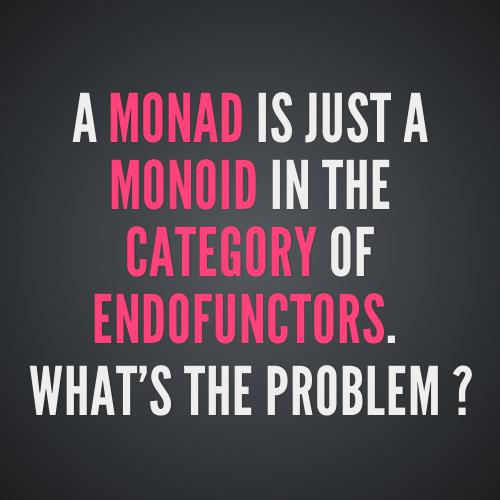
\includegraphics[height=0.9\textheight]{monad-is}}
\end{frame}

\begin{frame}[fragile]
  \frametitle{Kleisli category}
  \begin{itemize}
    \item Kleisli categories formalise monadic composition
  \item For any monad $T$ over a category $\mathcal{C}$, the \alert{Kleisli category} of $\mathcal{C}$, written $\mathcal{C}_T$ is a category with the same objects as $\mathcal{C}$, but with morphisms given by:
    \begin{itemize}
    \item $\operatorname{hom}_{\mathcal{C}_T}(x,y) = \operatorname{hom}_\mathcal{C}(x,T(y)),\ \forall x,y\in\operatorname{ob}(\mathcal{C})$
    \end{itemize}
  \item The identity morphisms in $\mathcal{C}_T$ are given by $\operatorname{id}_x = \eta(x), \forall x$, and morphisms $f: x\longrightarrow T(y)$ and $g: y\longrightarrow T(z)$ in $\mathcal{C}$ can compose to form $g\, \circ_T f : x\longrightarrow T(z)$ via
    \begin{itemize}
      \item $g\ \circ_T f = \mu_z \circ T(g) \circ f$
    \end{itemize}
    leading to composition of morphisms in $\mathcal{C_T}$.
    \item In FP, the morphisms in $C_T$ are often referred to as \alert{Kleisli arrows}, or \alert{Kleislis}, or sometimes just \alert{arrows} (although \alert{Arrow} usually refers to a generalisation of Kleisli arrows, sometimes known as \alert{Hughes arrows})
  \end{itemize}
\end{frame}

\begin{frame}
\centerline{
\includegraphics[height=0.9\textheight]{say-monad}}
\end{frame}

\subsection{Scalable modelling and computation}

\begin{frame}[fragile]
  \frametitle{Apache Spark}
  \begin{itemize}
  \item We have already seen how parallel monadic collections can automatically parallelise ``map'' and ``reduce'' operations
  \item \alert{Apache Spark} is a Scala library for Big Data analytics on (large) clusters of machines (in the cloud)
  \item The basic datatype provided by Spark is an \alert{RDD} --- a resilient distributed dataset
  \item An RDD is just a \alert{lazy}, \alert{distributed}, parallel monadic collection, supporting methods such as |map|, |flatMap|, |reduce|, etc., which can be used in exactly the same way as any other monadic collection
    \item Code looks exactly the same whether the RDD is a small dataset on a laptop or terabytes in size, distributed over a large Spark cluster
  \end{itemize}
\end{frame}

\begin{frame}[fragile]
  \frametitle{Laziness, composition, laws and optimisations}
  \begin{itemize}
    \item Laziness allows some optimisations to be performed that would be difficult to automate otherwise
    \item Consider a dataset |rdd: RDD[T]|, functions |f: T => U|, |g: U => V|, and a binary operation |op: (V,V) => V| for monoidal type |V|
    \item We can map the two functions and then reduce with:
      \begin{itemize}
      \item |rdd map f map g reduce op|
        \item to get a value of type |V|, all computed in parallel
      \end{itemize}
    \item However, re-writing this as:
      \begin{itemize}
      \item |rdd map (g compose f) reduce op|
        \item would eliminate an intermediate collection, but is equivalent due to the 2nd functor law
      \end{itemize}
      \item Category theory \alert{laws} often correspond to \alert{optimisations} that can be applied to code without affecting results --- Spark can do these optimisations \alert{automatically} due to lazy evaluation
  \end{itemize}
\end{frame}


\begin{frame}[fragile]
  \frametitle{Distributed computation}
  \begin{itemize}
  \item Big data frameworks such as Spark have been developed for the analysis of huge (internet scale) datasets on large clusters in the cloud
  \item They typically work by layering on top of a distributed file system (such as HDFS) which distributes a data set across a cluster and leaves data in place, sending required computation across the network to the data
    \item With a little thought, it is clear that even in the case of ``small data'' but ``big models''/``big computation'', these frameworks can be exploited for distributing computation
  \end{itemize}
\end{frame}

\begin{frame}[fragile]
  \frametitle{Typeclasses}
  \begin{itemize}
  \item \alert{Typeclasses} are a mechanism for supporting \alert{ad hoc polymorphism} in (functional) programming languages
  \item They are more flexible way to provide polymorphic functionality than traditional inheritance-based object classes in conventional object-oriented programming languages
  \item To define a typeclass (such as |Monoid|) for a basic type, the language must support \alert{parametric types}
  \item To define a typeclass (such as |Functor| or |Monad|) for a parametric type or type constructor, the language must support \alert{higher-kinded types} (very few widely-used languages do)
  \end{itemize}
\end{frame}


\begin{frame}[fragile]
  \frametitle{Typeclasses for Monoid, Functor and Monad}
  \begin{itemize}
  \item In Scala, we can define typeclasses for |Monoid|, |Functor| and |Monad| (using parametric and higher-kinded types):
  \end{itemize}
  \begin{lstlisting}[language=scala]
  trait Monoid[A] {
    def combine(a1: A, a2: A): A
    def id: A
  }
    
  trait Functor[F[_]] {
    def map[A,B](fa: F[A])(f: A => B): F[B]
  }

  trait Monad[M[_]] extends Functor[M] {
    def unit[A](a: A): M[A]
    def flatMap[A,B](ma: M[A])(f: A => M[B]): M[B]
  }
\end{lstlisting}
\end{frame}

\begin{frame}[fragile]
  \frametitle{A generic collection typeclass}
  \begin{itemize}
  \item We can define a typeclass for generic monadic collections:
\begin{lstlisting}[language=scala]
trait GenericColl[C[_]] {
  def map[A,B](ca: C[A])(f: A => B): C[B]
  def reduce[A](ca: C[A])(f: (A, A) => A): A
  def flatMap[A,B,D[B] <: GenTraversable[B]](
                 ca: C[A])(f: A => D[B]): C[B]
  def zip[A,B](ca: C[A])(cb: C[B]): C[(A, B)]
  def length[A](ca: C[A]): Int
}
\end{lstlisting}
and then define instances for standard collections (eg. |Vector|), parallel collections (eg. |ParVector|), and distributed parallel collections (eg. |RDD|)
\item We can then write code that is completely \alert{parallelisation--agnostic}
  \end{itemize}
\end{frame}

\begin{frame}[fragile]
  \frametitle{A scalable particle filter}
Single--observation update of a bootstrap particle filter:
\begin{lstlisting}[language=scala]
def update[S: State, O: Observation,
                        C[_]: GenericColl](
    dataLik: (S, O) => LogLik, stepFun: S => S
       )(x: C[S], o: O): (LogLik, C[S]) = {
  val xp = x map (stepFun(_))
  val lw = xp map (dataLik(_, o))
  val max = lw reduce (math.max(_, _))
  val rw = lw map (lwi => math.exp(lwi - max))
  val srw = rw reduce (_ + _)
  val l = rw.length
  val z = rw zip xp
  val rx = z flatMap (p => Vector.fill(
            Poisson(p._1 * l / srw).draw)(p._2))
  (max + math.log(srw / l), rx)
}  
\end{lstlisting}
\end{frame}

\begin{frame}[fragile]
  \frametitle{Filtering as a functional fold}
  \begin{itemize}
  \item Once we have a function for executing one step of a particle filter, we can produce a function for particle filtering as a functional fold over a sequence of observations:
  \end{itemize}
\begin{lstlisting}[language=scala]
def pFilter[S: State, O: Observation,
    C[_]: GenericColl, D[O] <: GenTraversable[O]](
    x0: C[S], data: D[O], dataLik: (S, O) => LogLik,
    stepFun: S => S ): (LogLik, C[S]) = {
  val updater = update[S, O, C](dataLik, stepFun) _
  data.foldLeft((0.0, x0))((prev, o) => {
    val next = updater(prev._2, o)
    (prev._1 + next._1, next._2)
  })
}
\end{lstlisting}
Again, completely parallelisation--agnostic...
\end{frame}

\begin{frame}[fragile]
  \frametitle{Scalable statistical modelling}
  \begin{itemize}
  \item We have looked a lot at scalable statistical \alert{computation}, but what about scalable statistical \alert{modelling} more generally?
  \item Independently of any computational issues, statistical modelling of large, complex problems is all about structure, modularity and composition --- again, the domain of category theory...
  \item When Bayesian hierarchical modelling, we often use \alert{probabilistic programming languages} (such as BUGS, JAGS, Stan...) to build up a large, complex (DAG) model from simple components
    \item It turns out that \alert{monads}, and especially \alert{free monads}, can give us a different (better?) perspective on building and inferring probabilistic models
  \end{itemize}
\end{frame}

\begin{frame}[fragile]
  \frametitle{Composing random variables with the probability monad}
  \begin{itemize}
  \item The \alert{probability monad} provides a foundation for describing random variables in a pure functional way
  \item We can build up joint distributions from marginal and conditional distributions using \alert{monadic composition}
  \item For example, consider an exponential mixture of Poissons (marginally negative binomial): we can think of an exponential distribution parametrised by a rate as a function |Exponential: Double => Rand[Double]| and a Poisson parametrised by its mean as a function |Poisson: Double => Rand[Int]|
    \item Those two functions don't directly compose, but do in the Kleisli category of the |Rand| monad, so |Exponential(3) flatMap {Poisson(_)}| will return a |Rand[Int]| which we can draw samples from if required
  \end{itemize}
\end{frame}


\begin{frame}[fragile]
  \frametitle{Monads for probabilistic programming}
  \begin{itemize}
    \item For larger probability models we can use \alert{for-comprehensions} to simplify the model building process, eg.
\begin{lstlisting}[language=scala]
  for { mu <- Gaussian(10,1)
        tau <- Gamma(1,1)
        sig = 1.0/sqrt(tau)
        obs <- Gaussian(mu,sig) }
  yield ((mu,tau,obs))
\end{lstlisting}
  \item We can use a regular probability monad for building forward models this way, and even for building models with simple Bayesian inference procedures allowing conditioning
    \item For sophisticated probabilistic sampling algorithms (eg. SMC, MCMC, pMCMC, HMC, ...) it is better to build models like this using a \alert{free monad} which can be \alert{interpreted} in different ways
  \end{itemize}
\end{frame}

\section{Summary and conclusions}

\subsection{Summary}

\begin{frame}
  \frametitle{Summary}
  \begin{itemize}
  \item You can't learn much about either FP or CT in a single talk/seminar
  \item I don't expect everyone to have understood everything!
  \item The aim was to give a little insight into:
    \begin{itemize}
    \item Why FP is interesting, and inherently more modular, composable and scalable than imperative programming
    \item Why CT is a good model for composable computation (because it is a theory of structure and composition)
      \item Why CT provides powerful abstractions which make FP easier, more modular, and more general
      \end{itemize}
  \end{itemize}
\end{frame}

\subsection{Conclusions}

\frame{
  \frametitle{Conclusions}
  \begin{itemize}
  \item We should approach the problem of statistical modelling and computation in a modular, composable, functional way, guided by underpinning principles from category theory
  \item To implement solutions to problems in statistical modelling and computation in a more scalable way, we need programming languages which are:
    \begin{itemize}
    \item \alert{Strongly statically typed}
    \item \alert{Compiled}
    \item \alert{Functional}
      \item and support \alert{typeclasses} and \alert{higher-kinded types}
    \end{itemize}
  \item \alert{Scala} and \alert{Spark} provide a nice illustration of the power of this approach, but there are other interesting languages, including: Haskell, (S)ML, OCaml, Frege, Eta, ...
    \item For more about Scala: \alert{\url{darrenjw.wordpress.com}}
  \end{itemize}
  }


\end{document}

